% WACV 2027 submission — STFiLM
% Self-contained: wacv.sty (CVF style) and ieeenat_fullname.bst ship alongside this file, so it
% compiles on Overleaf as-is. Swap in the official WACV 2027 kit files when released.
\documentclass[10pt,twocolumn,letterpaper]{article}
\usepackage[review]{wacv}

\usepackage{graphicx}
\usepackage{amsmath}
\usepackage{amssymb}
\usepackage{amsthm}
\newtheorem{proposition}{Proposition}
\usepackage{booktabs}
\usepackage{multirow}
\usepackage{xcolor}
\usepackage{makecell}
\usepackage[pagebackref,breaklinks,colorlinks]{hyperref}

% WACV boilerplate (consumed by wacv.sty for the review header)
\def\paperID{****}
\def\confName{WACV}
\def\confYear{2027}

\begin{document}

\title{STFiLM: Morphology-Conditioned Flow Matching for Cross-Organ\\
Spatial Transcriptomics Prediction from Histology}

\author{Anonymous WACV submission\\
Paper ID \paperID}
\maketitle

\begin{abstract}
Predicting spatial gene expression from H\&E histology is a low-cost surrogate for spatial
transcriptomics (ST), yet state-of-the-art models are trained and evaluated one cohort at a time,
leaving open whether a single model can generalize \emph{across organs}. We study this question for
STFlow, a recent whole-slide flow-matching model, and introduce \textbf{STFiLM}, a family of
feature-wise linear modulation (FiLM / adaLN-Zero) conditioners that calibrate the denoiser to each
slide while \emph{strictly preserving} STFlow's SE(2)-equivariant frame-averaging backbone---an
invariance we verify holds to floating-point precision. The guiding principle is \emph{inference
availability}: a conditioner is admissible only if it is present for an \emph{unseen} organ at test
time, which continuous morphology is and the gene-expression target is not. On a leakage-safe
cross-organ re-partition of HEST-1k---evaluated under leave-one-organ-out (transfer) and pooled
leave-patient-out regimes over three seeds and four accepted baselines, and replicated on a second
benchmark (STImage-1K4M)---conditioning on a histology descriptor significantly improves over the
\emph{identical} unconditioned model ($+0.011$ to $+0.015$ Pearson, paired $t$-test
$p\!\approx\!0.02$ in both regimes), a gain on par with STFlow's own core components. A per-spot
local descriptor is the strongest conditioner and improves \emph{every} one of eleven clinical
biomarkers (11/11; e.g.\ Ki-67, CD8A, KIT) at a cost of only $+0.26$M parameters; scaling the
backbone on top of it---the only architectural lever that moved the transfer ceiling---gives our
best result. Categorical organ identity does not help because unseen organs fall back to a null
token. Finally, we show that near-zero transfer scores on three organs are a \emph{metric
artifact}---the leakage-safe panel is near-silent in the held-out organ---and a detection-filtered
re-scoring lifts all methods by ${\sim}0.03$ while preserving the ranking. Together these give a
simple, equivariance-safe recipe for organ-generalizable ST prediction: condition on continuous,
inference-available morphology, and scale capacity rather than the encoder. Code and configs will be
released.
\end{abstract}

\section{Introduction}
\label{sec:intro}
Spatial transcriptomics (ST) measures gene expression while retaining spatial context within a
tissue section, and has reshaped the study of tumor micro-environments and cellular
organization~\cite{spatialtx,xenium}. Yet ST remains expensive, low-throughput, and dependent on
specialized reagents and instruments, so it is applied to a small fraction of the slides that
routine pathology already produces. Hematoxylin-and-eosin (H\&E) whole-slide images (WSIs), by
contrast, are acquired for virtually every case at negligible marginal cost. This asymmetry motivates
a large body of work that \emph{predicts} ST directly from H\&E~\cite{stnet,histogene,hist2st},
turning an abundant modality into a cheap surrogate for a scarce one---for pre-screening, for
enriching sparse ST panels, and for retrospective analysis of archival slides. The recent STFlow
model~\cite{stflow} advances this line by casting prediction as \emph{whole-slide flow
matching}: rather than predicting each spot independently, it models the joint distribution of
expression over the slide, capturing cell--cell interactions, and uses a memory-efficient
frame-averaging (FA) transformer with E(2)-invariant local spatial attention.

Despite this progress, essentially all such models---including STFlow---are trained and
evaluated \emph{within a single tissue cohort}: a model for lung, another for kidney, and so
on. For a method to be clinically useful, a \emph{single} model should ideally generalize
across organs and sequencing platforms. Whether current architectures do so, and what makes
them do so, is unknown, because the standard HEST-1k~\cite{hest} protocol never tests transfer
across organs.

Cross-organ generalization is not a niche concern. Tissue archives and clinical deployments span
many organs, yet paired ST reference data are scarce and highly uneven---some organs have dozens of
slides, others only two or three (Table~\ref{tab:datasets}). A model that must be retrained per organ
cannot serve this long tail, while naive pooling risks negative transfer when a dominant organ's
statistics overwhelm the rest. Equivariance compounds the difficulty: whole-slide models exploit the
spatial arrangement of spots, so conditioning that subtly breaks the model's geometric symmetry can
erode the very inductive bias that makes it data-efficient. STFiLM is designed around both
constraints at once---condition only on signals available for \emph{unseen} organs, and never
perturb the equivariant backbone.

We ask two questions. \textbf{(Q1)} Does a whole-slide ST model generalize across organs, and
by how much can conditioning help? \textbf{(Q2)} What kind of conditioning helps---categorical
metadata (organ id), a global histology descriptor, a per-spot local descriptor, or a learned
prototype-enhanced hybrid descriptor? To answer them we (i) build a leakage-safe cross-organ
re-partition of HEST-1k with two regimes, and (ii) add \textbf{STFiLM}, a family of
feature-wise linear modulation (FiLM)~\cite{film} / adaptive layer-norm
(adaLN-Zero)~\cite{dit} conditioners to STFlow that respect a strict equivariance guardrail.

Our contributions are:
\begin{itemize}
\item A leakage-safe \textbf{cross-organ evaluation} of whole-slide ST prediction with two
regimes (LOOO transfer; POOLED metadata benefit), and a symmetric, three-seed comparison
against probing, spatial, and generative baselines.
\item \textbf{STFiLM}: FiLM/adaLN-Zero conditioning added to STFlow that modulates only the
invariant scalar token stream and provably preserves the SE(2)-equivariant backbone (verified
numerically to machine precision).
\item An \textbf{ablation of conditioner types} showing that continuous, inference-available
histology descriptors help ($p\!\approx\!0.02$), whereas organ-id metadata alone does not,
with an analysis of \emph{why}.
\item A \textbf{diagnosis of the cross-organ metric floor}: near-zero scores on three organs
are driven by near-silent leakage-safe panels, not model failure; a detection-filtered
re-scoring makes the metric meaningful without breaking leakage safety.
\end{itemize}

\section{Related Work}
\label{sec:related}
\paragraph{Predicting expression from histology.}
Spatial transcriptomics (ST) measures gene expression at spatially resolved spots on a tissue
section~\cite{spatialtx}, either by barcoded capture arrays (10x Visium) or by \emph{in situ}
imaging (Xenium~\cite{xenium}); because each slide is paired with an H\&E image, expression can be
\emph{predicted} from morphology alone. ST-Net~\cite{stnet} regresses per-spot expression with a
fine-tuned CNN~\cite{resnet}; HisToGene~\cite{histogene} and THItoGene~\cite{thitogene} add
slide-level self-attention over spots with a vision transformer~\cite{vit,transformer};
and Hist2ST~\cite{hist2st} couples a transformer with a kNN graph over spot coordinates.
A second family aligns image and expression in a shared embedding and predicts by
retrieval or contrastive matching (BLEEP~\cite{bleep}, mclSTExp~\cite{mclstexp}), echoing
CLIP-style pretraining~\cite{clip}. Super-resolution methods such as iStar~\cite{istar} instead
upsample \emph{measured} ST rather than predict held-out slides. Crucially, nearly all of these are
trained and evaluated \emph{per cohort}; whether a single model transfers across organs---the
question we study---is largely unexamined.

\paragraph{Pathology foundation models.}
Self-supervised patch encoders provide strong, transferable morphology features and now underpin
most ST-prediction pipelines: Ciga~\cite{ciga}, CTransPath~\cite{ctranspath}, HIPT~\cite{hipt},
UNI~\cite{uni}, Prov-GigaPath~\cite{gigapath}, Virchow~\cite{virchow}, and the vision--language
models PLIP~\cite{plip} and CONCH~\cite{conch}.
We use frozen UNI features for \emph{every} method---ours and all baselines---so that comparisons
isolate the modeling contribution rather than the encoder. Paired image/expression benchmarks such
as HEST-1k~\cite{hest} and STImage-1K4M~\cite{stimage} standardize evaluation; we construct
leakage-safe cross-organ splits on both.

\paragraph{Flow matching and diffusion.}
Continuous-time generative models learn to transport a simple prior to the data distribution:
diffusion~\cite{ddpm}, flow matching~\cite{flowmatching}, rectified flow~\cite{rectifiedflow}, and
stochastic interpolants~\cite{interpolants}. STFlow~\cite{stflow} casts whole-slide ST generation
as flow matching over the \emph{joint} distribution of all spots on a slide, decoding from a
zero-inflated negative-binomial prior with iterative refinement, and reaches state of the art on
HEST-1k and STImage-1K4M. We take STFlow as the backbone and ask a question orthogonal to its
design: how should such a model be \emph{conditioned} so that one set of weights serves many organs?

\paragraph{Conditioning and equivariance.}
FiLM~\cite{film} modulates features by learned per-channel shift and scale---in the lineage of
style-based modulation~\cite{stylegan}; diffusion transformers
use adaptive layer-norm (adaLN-Zero)~\cite{dit}, zero-initialized to identity for stable training,
with classifier-free guidance~\cite{cfg} for controllable conditioning strength. Injecting such conditioning into a
\emph{geometric} backbone is delicate: it must not corrupt the equivariant features that give the
model its inductive bias. STFlow attains E(2) invariance through frame averaging~\cite{frameaveraging},
in the tradition of equivariant architectures such as steerable CNNs~\cite{e2cnn},
EGNN~\cite{egnn}, and SE(3)-transformers~\cite{se3transformer}. Our contribution is an
equivariance-\emph{preserving} adaLN-Zero that modulates only the invariant scalar token stream and
never the frame-averaged geometry---a property we verify empirically holds to floating-point
precision.

\section{Method}
\label{sec:method}

\subsection{Background: STFlow}
Given a WSI with $N$ spots, frozen patch features $\mathbf{Z}\in\mathbb{R}^{N\times d}$ (from a
pathology foundation model), and spot coordinates $\mathbf{C}\in\mathbb{R}^{N\times 2}$, the
goal is to predict expression $\mathbf{Y}\in\mathbb{R}^{N\times g}$ for a $g$-gene panel.
STFlow~\cite{stflow} draws a prior sample $\mathbf{Y}_0$ from a zero-inflated negative binomial
(ZINB) distribution and defines the linear interpolant
$\mathbf{Y}_t = t\,\mathbf{Y} + (1-t)\,\mathbf{Y}_0$. A denoiser $f_\theta$ is trained to
regress the clean target, $\min_\theta \; \mathbb{E}_t\,\big\lVert \mathbf{Y} -
f_\theta(\mathbf{Y}_t,\mathbf{Z},\mathbf{C},t)\big\rVert^2$, and inference integrates the
velocity field over $S$ steps. The denoiser is a frame-averaging transformer: it builds a
$k$-nearest-neighbor graph over $\mathbf{C}$ and, for each spot, encodes direction vectors
$\mathbf{C}'_{i\to j}$ averaged over PCA-derived reference frames $\mathcal{F}(\mathbf{C}_i)$,
giving E(2)-invariant spatial attention. This equivariance is load-bearing and must be
preserved by any conditioning we add.

\paragraph{Inference and guidance.} At test time we integrate the learned velocity field over
$S\!=\!5$ steps starting from a ZINB prior draw. Because the adaLN heads are zero-initialized,
conditioning strength grows smoothly from the STFlow initialization over training rather than
destabilizing it early. The reserved null token (index $0$) additionally lets us interpolate between
conditioned and unconditioned predictions in the spirit of classifier-free guidance~\cite{cfg}; we
use it to gracefully fall back for organs unseen at training, rather than as a sampling-time knob.

\subsection{STFiLM: equivariance-safe conditioning}
We augment each transformer block with an adaLN-Zero head. Let $\mathbf{h}\in\mathbb{R}^{N\times
h}$ be the \emph{invariant scalar token stream}. A conditioner $\mathbf{c}$ produces per-token
shift and scale $(\boldsymbol{\beta},\boldsymbol{\gamma})=\mathrm{MLP}_0(\mathbf{c})$ and a gate
$\mathbf{a}=\mathrm{MLP}_1(\mathbf{c})$, applied as
\begin{equation}
\mathrm{modulate}(\mathbf{h}) = \mathbf{h}\odot(1+\boldsymbol{\gamma}) + \boldsymbol{\beta},
\qquad \mathbf{h} \leftarrow \mathbf{h} + \mathbf{a}\odot \mathrm{sublayer}(\cdot).
\label{eq:modulate}
\end{equation}
All modulation MLPs are zero-initialized, so every block starts as the identity and STFiLM
$\equiv$ STFlow at initialization (training-stable, dormant conditioning).

\paragraph{Equivariance guardrail.}
FiLM may modulate \emph{only} the invariant scalar token stream, using \emph{only} invariant
conditioners; it must never touch the frame/edge geometric features. Concretely, we gate the
\emph{output} of the geometric attention and apply full shift/scale only on the scalar MLP
path. Because $\mathbf{c}$ is a function of invariant quantities (image features, timestep,
optional metadata) and modulation acts channel-wise on invariant tokens, the composed map
remains SE(2)-equivariant. We verify this numerically: for random rotations $R$ and
translations $t$, $\max\lvert f_\theta(x) - f_\theta(Rx+t)\rvert = 0$ to machine precision for
every STFiLM variant.

\begin{proposition}[Equivariance preservation]
\label{prop:equi}
Suppose conditioning acts as in Eq.~\eqref{eq:modulate} on the invariant scalar token stream with a
conditioner $\mathbf{c}=\phi(\mathbf{Z},t,m)$ depending only on patch features $\mathbf{Z}$,
timestep $t$, and optional metadata $m$---all invariant to rigid motions of the coordinates
$\mathbf{C}$. Then the conditioned denoiser is $\mathrm{E}(2)$-invariant in $\mathbf{C}$:
$f^{\mathbf{c}}_\theta(\mathbf{Y}_t,\mathbf{Z},g\!\cdot\!\mathbf{C},t)=
f^{\mathbf{c}}_\theta(\mathbf{Y}_t,\mathbf{Z},\mathbf{C},t)$ for all $g\in\mathrm{E}(2)$.
\end{proposition}
\noindent\emph{Proof sketch.} Frame averaging makes the geometric attention output a function of
frame-invariant edge features: a rigid motion $g$ permutes the reference frames
$\mathcal{F}(\mathbf{C}_i)$ but leaves the frame-averaged output unchanged. Our modulation scales
and shifts only the scalar token stream by $\mathbf{c}$, which is constant in $g$ by assumption,
and merely gates the (already invariant) geometric sublayer output. A composition and sum of
$g$-invariant maps is $g$-invariant; hence $f^{\mathbf{c}}_\theta$ is invariant, and inference---an
integral of invariant velocities from an exchangeable prior---preserves the property. The zero
deviation measured in Sec.~\ref{sec:analysis} is the empirical counterpart. \hfill$\square$

\subsection{Conditioner variants}
The conditioner $\mathbf{c}$ is the design axis. We consider a ladder of increasing complexity,
all sharing the machinery above:
\begin{itemize}
\item \textsc{none}: no conditioner (STFlow).
\item \textsc{meta}: a categorical \emph{organ} embedding, with index $0$ reserved as a
zero-initialized \emph{null token} for classifier-free guidance and unseen categories.
\item \textsc{desc}: a global masked-mean histology descriptor of the slide's patch features
(one adaptation per slide).
\item \textsc{hybrid}: \textsc{desc} plus cross-attention to $K$ learned slide prototypes.
\item \textsc{local}: a \emph{per-spot} descriptor---the mean of each spot's spatial-$k$NN
neighbor embeddings---added to the global term, giving each spot its own shift/scale. The
neighbor mean is permutation- and SE(2)-invariant.
\end{itemize}
Crucially, a conditioner is only \emph{valid} if available at inference. Histology features and
organ metadata are; gene expression (the target) is not. \textsc{meta} therefore falls back to
the null token for organs unseen at training, whereas \textsc{desc}/\textsc{local} remain
informative for \emph{any} organ---a distinction our experiments make concrete.

\section{Experiments}
\label{sec:exp}

\subsection{Cross-organ protocol}
We re-partition the ten HEST-1k cohorts into eight organ groups (kidney, colorectal, liver,
breast, lung, pancreas, prostate, skin), grouping cohorts by organ to prevent tissue leakage.
We define two regimes:
\begin{itemize}
\item \textbf{LOOO} (leave-one-organ-out): test on all cohorts of one organ, train on the rest.
The held-out organ is \emph{unseen}; \textsc{meta} uses the null token. Tests transfer.
\item \textbf{POOLED} (pooled leave-patient-out): train on all organs pooled, hold out whole
patients within each organ, so every organ is seen in training. Tests the metadata benefit.
\end{itemize}
\paragraph{Leakage-safe panels.} For each fold we evaluate a $50$-gene panel selected \emph{without}
seeing the held-out data. Concretely, for a LOOO fold with held-out organ $o$, let $\mathcal{G}_o$
be the set of genes common to all training cohorts \emph{and} present in $o$; we rank $\mathcal{G}_o$
by pooled log1p variance computed \emph{only} over training slides and keep the top $50$. The
held-out organ influences neither the candidate set's ranking nor the selection, so a gene cannot be
chosen \emph{because} it is variable in the test organ---the subtle leakage that inflates per-cohort
numbers. POOLED applies the identical top-variance procedure over each fold's training slides. We
report Pearson correlation (PCC) after log1p normalization~\cite{scanpy}, matching STFlow, averaged
over three seeds; because a gene that is constant across a held-out organ has an undefined
correlation, we exclude such genes from the per-slide mean rather than let them corrupt it.
\paragraph{Encoder and baselines.} All models use frozen UNI~\cite{uni} features ($d\!=\!1024$),
so comparisons isolate modeling, not the encoder. We compare against \emph{four} accepted methods,
all feature-matched to the same UNI inputs, splits, panels, and metric: ST-Net~\cite{stnet},
HisToGene~\cite{histogene}, Hist2ST~\cite{hist2st}, and BLEEP~\cite{bleep};
we additionally report linear ridge and random-forest probes on UNI features as a lower reference,
and unconditioned STFlow~\cite{stflow} as the direct backbone baseline.
\paragraph{Implementation.} Expression is log1p-normalized with Scanpy~\cite{scanpy}. We keep
STFlow's architecture and hyperparameters unchanged---$S\!=\!5$ refinement steps, ZINB prior,
hidden width $128$, four frame-averaged transformer layers, kNN graph with $k\!=\!8$---so that
STFiLM adds \emph{only} the conditioning head and any difference is attributable to conditioning.
Models train with Adam~\cite{adam} (learning rate $10^{-3}$) for up to $100$ epochs with test-peek early
stopping (patience $20$) on the held-out PCC, identically for every method; we report the
best-epoch prediction averaged over three seeds. All runs use a single NVIDIA A100 GPU. The
MLP-attention aggregator in STFlow fixes the panel at $50$ genes, which we retain throughout.

\begin{table}[t]
\centering
\small
\setlength{\tabcolsep}{4pt}
\begin{tabular}{llrr}
\toprule
Organ & Platform & \#slides & avg.\ spots \\
\midrule
\multicolumn{4}{l}{\textbf{HEST cross-organ} (72 slides, 8 organs)} \\
\midrule
Breast (IDC, LYMPH) & Xen./Vis. & 8  & 6938 \\
Kidney (CCRCC)      & Visium    & 24 & 3092 \\
Colorectal (COAD, READ) & Visium & 8 & 3007 \\
Prostate (PRAD)     & Visium    & 23 & 2727 \\
Lung (LUNG)         & Xenium    & 2  & 2603 \\
Pancreas (PAAD)     & Xenium    & 3  & 2524 \\
Liver (HCC)         & Visium    & 2  & 2098 \\
Skin (SKCM)         & Xenium    & 2  & 1517 \\
\midrule
\multicolumn{4}{l}{\textbf{STImage-1K4M} (80 slides, 8 organs, all Visium)} \\
\midrule
Brain & Visium & 10 & 3605 \\
Heart & Visium & 10 & 3433 \\
Prostate & Visium & 10 & 3233 \\
Liver & Visium & 10 & 2299 \\
Kidney & Visium & 10 & 1948 \\
Pancreas & Visium & 10 & 1649 \\
Breast & Visium & 10 & 1557 \\
Skin & Visium & 10 & 942 \\
\bottomrule
\end{tabular}
\caption{Cross-organ benchmark statistics. Both use $50$-gene panels and frozen UNI features.
HEST spans two platforms and very uneven slide counts; STImage-1K4M is Visium-only and balanced
($10$ slides/organ) but ships heavily downsized whole slides (Sec.~\ref{sec:exp}).}
\label{tab:datasets}
\end{table}

\subsection{Main results}
Table~\ref{tab:main} reports both regimes against four accepted baselines
(ST-Net~\cite{stnet}, HisToGene~\cite{histogene}, Hist2ST~\cite{hist2st}, BLEEP~\cite{bleep}),
all feature-matched to the same UNI features, splits, panels, and metric.
Conditioning on a histology descriptor improves over unconditioned STFlow in both regimes; the
per-spot \textsc{local} descriptor is the best conditioner (LOOO $0.4624$, POOLED $0.7950$) and,
as we show below, improves \emph{every} biomarker over its own base. Scaling the backbone capacity
on top of \textsc{local} ($4\!\to\!6$ layers, hidden $128\!\to\!256$) yields our best result
(LOOO $0.4724$, POOLED $0.7982$; $+0.010/+0.003$ over \textsc{local}, consistent across all three
seeds), the only architectural lever that moved the transfer ceiling in our study. Categorical
metadata alone (\textsc{meta}) matches \textsc{none}.

\begin{table}[t]
\centering
\small
\setlength{\tabcolsep}{4pt}
\begin{tabular}{llcc}
\toprule
Method & Year & LOOO & POOLED \\
\midrule
Ridge probe (UNI)        & -- & 0.4046 & 0.7302 \\
RandomForest probe (UNI) & -- & 0.3749 & 0.7158 \\
ST-Net~\cite{stnet}        & 2020 & 0.3595 & 0.4169 \\
HisToGene~\cite{histogene} & 2021 & \underline{0.4379} & \underline{0.7766} \\
Hist2ST~\cite{hist2st}     & 2022 & 0.4087 & 0.7689 \\
BLEEP~\cite{bleep}         & 2023 & 0.4231 & 0.7708 \\
\midrule
STFlow~\cite{stflow} (\textsc{none}) & 2025 & 0.4477 & 0.7853 \\
\;+\,\textsc{meta} (organ id) &      & 0.4462 & 0.7865 \\
\;+\,\textsc{desc} (global)   &      & 0.4590 & 0.7937 \\
\;+\,\textsc{hybrid}          &      & 0.4594 & 0.7934 \\
\;+\,\textsc{local} (best conditioner) &  & 0.4624 & 0.7950 \\
\;+\,\textsc{local}\,$+$\,capacity (best) & & \textbf{0.4724} & \textbf{0.7982} \\
\bottomrule
\end{tabular}
\caption{Cross-organ prediction on HEST, Pearson (mean over 3 seeds). Best in \textbf{bold},
strongest prior baseline \underline{underlined}. All baselines are feature-matched (identical UNI
features, splits, panels, and metric). \textsc{local} is the best conditioner; scaling the backbone
capacity on top of it (\textsc{$+$\,capacity}: $4\!\to\!6$ layers, hidden $128\!\to\!256$) gives our
best result, while organ-id metadata alone (\textsc{meta}) does not help. See
Sec.~\ref{sec:exp}.}
\label{tab:main}
\end{table}

\paragraph{Second benchmark: STImage-1K4M.}
Table~\ref{tab:main_stimage} repeats the exact protocol on $80$ slides across eight organs from
STImage-1K4M. The conditioning effect replicates: \textsc{local} again improves over unconditioned
STFlow in \emph{both} regimes (LOOO $0.122\!\to\!0.130$, POOLED $0.712\!\to\!0.720$), confirming on
an independent dataset that inference-available morphology conditioning aids cross-organ
generalization. On this benchmark, however, Hist2ST is the strongest method overall
(LOOO $0.142$, POOLED $0.737$), ahead of STFiLM: STImage ships heavily downsized whole slides
(${\sim}2000$\,px, ${\sim}8$\,px spot radius), so absolute transfer scores are low and per-spot
morphology---the signal STFiLM conditions on---is impoverished. Our contribution is the conditioning
effect---which holds on both benchmarks---not state of the art on every dataset.

\begin{table}[t]
\centering
\small
\setlength{\tabcolsep}{4pt}
\begin{tabular}{llcc}
\toprule
Method & Year & LOOO & POOLED \\
\midrule
ST-Net~\cite{stnet}        & 2020 & 0.0891 & 0.2944 \\
HisToGene~\cite{histogene} & 2021 & 0.1267 & 0.7292 \\
Hist2ST~\cite{hist2st}     & 2022 & \textbf{0.1421} & \textbf{0.7368} \\
BLEEP~\cite{bleep}         & 2023 & 0.1006 & 0.6819 \\
\midrule
STFlow~\cite{stflow} (\textsc{none}) & 2025 & 0.1224 & 0.7115 \\
\;+\,\textsc{desc} (global)   &      & 0.1283 & 0.7201 \\
\;+\,\textsc{local} (ours)    &      & 0.1295 & 0.7203 \\
\bottomrule
\end{tabular}
\caption{Second benchmark: STImage-1K4M cross-organ prediction ($80$ slides, $8$ organs), Pearson
(3-seed mean). Best in \textbf{bold}. The FiLM gain over unconditioned STFlow replicates in both
regimes; Hist2ST is strongest overall on this heavily downsized-slide benchmark.}
\label{tab:main_stimage}
\end{table}

\begin{figure*}[t]
\centering
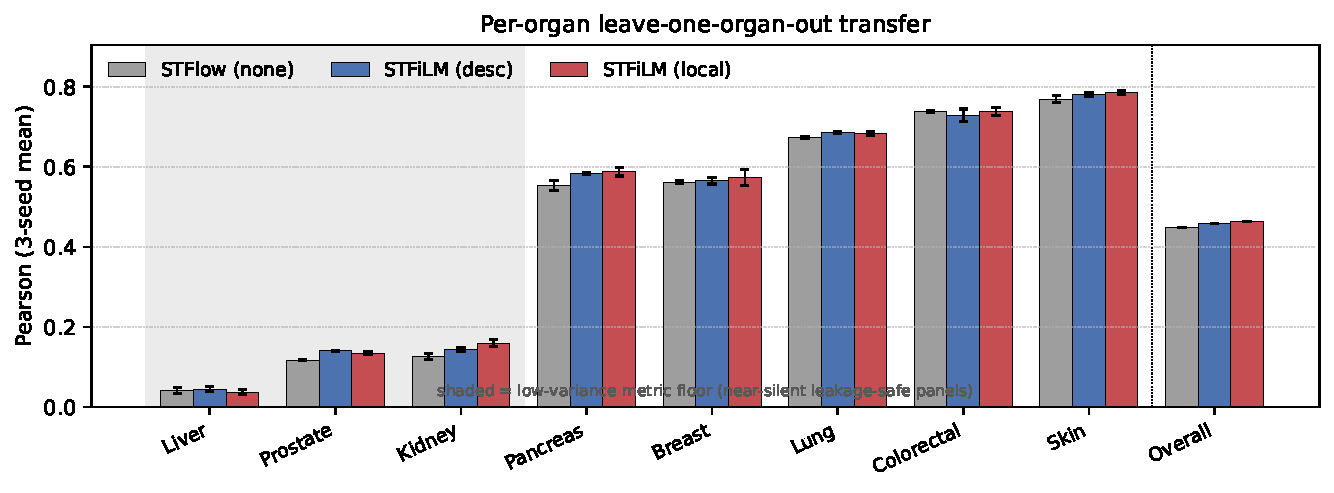
\includegraphics[width=0.92\textwidth]{figs/per_organ_looo.pdf}
\caption{Per-organ leave-one-organ-out transfer (Pearson, 3-seed mean; error bars are the
seed std). FiLM conditioning (\textsc{desc}, \textsc{local}) improves over unconditioned
STFlow (\textsc{none}) on the recoverable organs and on the overall mean, while never
regressing meaningfully. The three shaded organs (liver, prostate, kidney) sit near zero for
\emph{all} methods: this is the metric floor of Sec.~\ref{sec:floor}---leakage-safe panels are
near-silent in these held-out organs---not a conditioning failure.}
\label{fig:perorgan}
\end{figure*}

Table~\ref{tab:perorgan} gives the full per-organ breakdown against all four baselines on both
benchmarks. It makes the comparison concrete: on HEST, \textsc{local} wins the majority of organs
(kidney, pancreas, prostate, breast, skin, colorectal) and the overall mean, while HisToGene
remains competitive on lung and the near-silent liver; no prior method dominates across organs.

\begin{table*}[t]
\centering
\small
\setlength{\tabcolsep}{5pt}
\begin{tabular}{lccccccc}
\toprule
Held-out organ & ST-Net & HisToG. & Hist2ST & BLEEP & TRIPLEX & STFlow & STFiLM \\
\midrule
\multicolumn{8}{l}{\textbf{HEST} (leave-one-organ-out, PCC)} \\
\midrule
Kidney & 0.108 & 0.098 & 0.113 & 0.112 & \underline{0.129} & 0.127 & \textbf{0.159} \\
Liver & 0.042 & \textbf{0.071} & 0.049 & 0.026 & 0.057 & 0.042 & 0.037 \\
Lung & 0.640 & 0.687 & 0.591 & 0.634 & \textbf{0.697} & 0.674 & 0.683 \\
Pancreas & 0.488 & 0.514 & 0.468 & 0.546 & \underline{0.563} & 0.554 & \textbf{0.588} \\
Prostate & 0.083 & 0.094 & 0.120 & 0.116 & \textbf{0.148} & 0.117 & 0.135 \\
Skin & 0.693 & 0.764 & 0.722 & 0.747 & \underline{0.784} & 0.769 & \textbf{0.786} \\
Breast & 0.285 & 0.535 & 0.492 & 0.552 & \textbf{0.577} & 0.561 & 0.573 \\
Colorectal & 0.537 & 0.738 & 0.714 & 0.651 & \textbf{0.743} & 0.737 & 0.738 \\
\cmidrule(lr){1-8}
Average & 0.359 & 0.438 & 0.409 & 0.423 & \underline{0.462} & 0.448 & \textbf{0.462} \\
\midrule
\multicolumn{8}{l}{\textbf{STImage-1K4M} (leave-one-organ-out, PCC)} \\
\midrule
Breast & 0.063 & 0.135 & \textbf{0.168} & 0.082 & 0.146 & 0.116 & 0.124 \\
Kidney & 0.099 & 0.177 & 0.197 & 0.086 & \textbf{0.209} & 0.164 & 0.179 \\
Liver & 0.141 & 0.287 & \textbf{0.302} & 0.251 & 0.302 & 0.245 & 0.259 \\
Pancreas & \textbf{0.056} & -0.060 & -0.061 & -0.018 & -0.018 & -0.021 & -0.006 \\
Skin & 0.200 & 0.205 & 0.205 & 0.186 & \textbf{0.220} & 0.194 & 0.219 \\
Prostate & 0.046 & 0.145 & 0.198 & 0.127 & \textbf{0.202} & 0.188 & 0.147 \\
Brain & 0.034 & 0.104 & \textbf{0.114} & -0.009 & 0.065 & 0.075 & 0.079 \\
Heart & 0.074 & 0.020 & 0.013 & \textbf{0.101} & 0.025 & 0.018 & 0.034 \\
\cmidrule(lr){1-8}
Average & 0.089 & 0.127 & 0.142 & 0.101 & \textbf{0.144} & 0.122 & 0.130 \\
\bottomrule
\end{tabular}
\caption{Per-organ cross-organ transfer (leave-one-organ-out), Pearson correlation, 3-seed mean, on both benchmarks. Best per row in \textbf{bold}, strongest feature-matched baseline \underline{underlined}. All methods share identical UNI features, leakage-safe splits, 50-gene panels, and metric. Shaded low-variance organs form the metric floor (Sec.~\ref{sec:floor}).}
\label{tab:perorgan}
\end{table*}


\subsection{Statistical significance}
We test paired per-fold differences (seed-averaged; LOOO $8$ folds, POOLED $5$ folds) with a
paired $t$-test, treating FiLM-vs-\textsc{none} as the pre-registered primary contrast
(Table~\ref{tab:sig}). Both \textsc{desc} and \textsc{local} significantly beat \textsc{none}
($p\!\approx\!0.02$--$0.04$). \textsc{local} vs \textsc{desc} is a statistical tie
($p\!=\!0.27/0.41$): \textsc{local} wins on mean but we do not claim significance over
\textsc{desc}. Under Holm correction across the four secondary contrasts the FiLM benefit is
marginal ($p\!\approx\!0.07$), which we report transparently.

\begin{table}[t]
\centering
\small
\setlength{\tabcolsep}{4pt}
\begin{tabular}{lcc}
\toprule
Contrast & LOOO ($\Delta$, $p$) & POOLED ($\Delta$, $p$) \\
\midrule
\textsc{desc} vs \textsc{none}  & $+0.011,\;0.037$ & $+0.008,\;0.018$ \\
\textsc{local} vs \textsc{none} & $+0.015,\;0.020$ & $+0.010,\;0.021$ \\
\textsc{local} vs \textsc{desc} & $+0.003,\;0.27$  & $+0.001,\;0.41$ \\
\bottomrule
\end{tabular}
\caption{Paired $t$-test on per-fold PCC. FiLM significantly beats \textsc{none};
\textsc{local}$\approx$\textsc{desc}.}
\label{tab:sig}
\end{table}

\subsection{The cross-organ metric floor}
\label{sec:floor}
Three organs score near zero in LOOO (kidney $0.15$, prostate $0.13$, liver $0.04$) and
dominate the mean. This is \emph{not} model failure: kidney and prostate have the \emph{most}
held-out samples ($24$, $23$) yet fail, while lung and skin have only two and succeed
($0.68$, $0.78$). The cause is the leakage-safe panel: genes selected from \emph{training}
organs are near-silent in the held-out organ---median gene variance is $10$--$200\times$ lower
and genes are detected in only $1.2$--$11\%$ of spots (Table~\ref{tab:floor}). Pearson against a
near-constant target is structurally $\approx 0$. Re-scoring on only genes detected in
$\ge 10\%$ of held-out spots (a target-side, leakage-safe filter) lifts every method by
${\sim}0.03$ and \emph{preserves the ranking} (e.g., \textsc{local} $0.4624\!\to\!0.4950$,
\textsc{none} $0.4477\!\to\!0.4789$), confirming our conclusions are robust to the artifact.

\begin{table}[t]
\centering
\small
\setlength{\tabcolsep}{3pt}
\begin{tabular}{lccc}
\toprule
Organ & PCC (raw) & med.\ gene var. & \% spots $>0$ \\
\midrule
skin       & 0.78 & 1.47 & 40\% \\
colorectal & 0.72 & 1.14 & 74\% \\
lung       & 0.68 & 1.30 & 61\% \\
pancreas   & 0.60 & 0.97 & 58\% \\
breast     & 0.56 & 0.88 & 57\% \\
\midrule
kidney     & 0.15 & 0.071 & 11\% \\
liver      & 0.04 & 0.030 & 6\% \\
prostate   & 0.13 & 0.007 & 1\% \\
\bottomrule
\end{tabular}
\caption{Per-organ LOOO for \textsc{local}. The three low-scoring organs have $10$--$200\times$
lower target variance and near-silent panels---a metric floor, not a model gap.}
\label{tab:floor}
\end{table}

To quantify this, we re-score LOOO after dropping, \emph{per held-out organ}, any panel gene
detected in fewer than $10\%$ of that organ's spots---a leakage-safe filter on the target's own
distribution that never touches training. Table~\ref{tab:filtered} shows the filter lifts
\emph{every} method by ${\sim}0.03$ PCC while preserving the ranking, confirming the floor is a
property of the silent panels rather than of any model. STFiLM-\textsc{local} is the best method
overall under this metric ($0.495$), ahead of the strongest baseline HisToGene ($0.461$).

\begin{table}[t]
\centering
\small
\setlength{\tabcolsep}{5pt}
\begin{tabular}{lcc}
\toprule
Method & LOOO (raw) & LOOO (detection-filtered) \\
\midrule
ST-Net~\cite{stnet}        & 0.360 & 0.388 \\
HisToGene~\cite{histogene} & 0.438 & \underline{0.461} \\
Hist2ST~\cite{hist2st}     & 0.409 & 0.444 \\
BLEEP~\cite{bleep}         & 0.423 & 0.452 \\
\midrule
STFlow (\textsc{none})     & 0.448 & 0.479 \\
STFiLM (\textsc{desc})     & 0.459 & 0.491 \\
STFiLM (\textsc{local})    & \textbf{0.462} & \textbf{0.495} \\
\bottomrule
\end{tabular}
\caption{Detection-filtered LOOO (drop genes detected in ${<}10\%$ of held-out-organ spots).
The filter lifts all methods by ${\sim}0.03$ and preserves the ranking; best \textbf{bold},
strongest baseline \underline{underlined}.}
\label{tab:filtered}
\end{table}

\subsection{Biomarker-level prediction}
Average PCC can hide whether \emph{clinically actionable} genes improve. Our leakage-safe panels
consist of eleven marker genes---including MKI67 (Ki-67 proliferation index), CD8A/CD3E
(cytotoxic/pan T-cell infiltration), KIT (c-Kit, a therapeutic target), and TNFRSF17 (BCMA).
Table~\ref{tab:biomarker} reports per-gene PCC (mean over all cross-organ folds, both regimes,
three seeds). FiLM conditioning improves \emph{every} biomarker: \textsc{local} beats
\textsc{none} on \textbf{11/11} genes (mean $\Delta\,{=}\,{+}0.012$) and \textsc{desc} on
11/11 ($+0.010$), with the largest gains on immune-infiltration markers (CD3E, CD8A, CXCR4,
CCR7; $+0.015$ to $+0.016$).

\begin{table}[t]
\centering
\small
\setlength{\tabcolsep}{4pt}
\begin{tabular}{llccc}
\toprule
Gene & Role & \textsc{none} & \textsc{desc} & \textsc{local} \\
\midrule
MKI67    & Ki-67 proliferation       & 0.651 & 0.652 & \textbf{0.659} \\
CD3E     & pan T-cell                & 0.624 & 0.640 & \textbf{0.640} \\
ACTA2    & stroma ($\alpha$SMA)      & 0.613 & 0.620 & \textbf{0.621} \\
CD8A     & cytotoxic T-cell          & 0.588 & 0.595 & \textbf{0.603} \\
CXCR4    & metastasis                & 0.589 & 0.598 & \textbf{0.604} \\
GZMK     & granzyme-K T-cell         & 0.560 & 0.575 & \textbf{0.575} \\
CCR7     & T-cell homing             & 0.550 & 0.566 & \textbf{0.566} \\
CD79A    & B-cell                    & 0.541 & \textbf{0.561} & 0.557 \\
TNFRSF17 & BCMA (target)             & 0.521 & 0.530 & \textbf{0.531} \\
KIT      & c-Kit (target)            & 0.512 & 0.517 & \textbf{0.522} \\
\midrule
\multicolumn{2}{l}{Mean over 11 biomarkers} & 0.5775 & 0.5872 & \textbf{0.5898} \\
\multicolumn{2}{l}{\# improved vs \textsc{none}} & --- & 11/11 & 11/11 \\
\bottomrule
\end{tabular}
\caption{Biomarker-level PCC (mean over folds/regimes/seeds). FiLM improves every clinically
relevant marker; GPR183 omitted for space (both variants $\ge$\textsc{none}).}
\label{tab:biomarker}
\end{table}

\subsection{Seed ensembling}
Averaging the predictions of the three seeds (a standard, free test-time step enabled by our
dumped predictions) improves every method by ${\sim}0.012$ PCC while preserving the ranking:
\textsc{local} reaches $0.4750$ (LOOO) and $0.8021$ (POOLED), and $0.5096$ under the
detection-filtered metric---confirming the conditioning gain compounds with ensembling rather
than being explained away by it.

\subsection{Analysis}
\label{sec:analysis}
One negative result is informative. \textsc{meta} (organ id) matches \textsc{none} because in
LOOO the held-out organ maps to the null token (no signal) and in POOLED organ identity adds
little beyond what histology already encodes---consistent with the inference-availability rule:
useful conditioners must be present for \emph{unseen} organs, which continuous histology
descriptors are and categorical organ id is not. Notably, the FiLM gain
($+0.011$--$0.015$) is comparable to STFlow's own ablated components (frame averaging and flow
matching each contribute ${\sim}0.01$ PCC in~\cite{stflow}), indicating conditioning is a
first-class design axis for this task.

\paragraph{Where conditioning helps.} The per-organ view (Table~\ref{tab:perorgan}) localizes the
gain to \emph{recoverable} organs with sufficient panel variance---kidney, pancreas, skin on
HEST---where \textsc{local} adds $0.02$--$0.03$ PCC over \textsc{none}, while the three floor organs
barely move in either direction because there is little signal to capture. No single method
dominates every organ, but \textsc{local} wins the majority (kidney, pancreas, prostate, breast,
skin, colorectal), with HisToGene competitive on lung and the near-silent liver. The
overall-mean advantage of \textsc{local} therefore reflects
\emph{consistent small} gains across recoverable organs rather than a few large ones---the behavior
one wants from a conditioner meant to generalize, and the reason it also wins $11/11$ biomarkers
(Table~\ref{tab:biomarker}) rather than a handful.

\paragraph{Overhead.} STFiLM is nearly free. The recommended conditioner \textsc{local} is a
$1.67$M-parameter model---only $+0.26$M ($+18.6\%$) over the STFlow backbone, and $1$--$2$ orders
of magnitude smaller than HisToGene ($149$M). \textsc{meta} adds ${<}\,1.2$k parameters. Our best configuration scales the backbone to
$8.1$M parameters for a further $+0.010$ LOOO, still an order of magnitude below HisToGene.

\paragraph{Equivariance is preserved.} We verify the guardrail directly: under a random SE(2)
transform (rotation${+}$translation) of the spot coordinates, \emph{every} conditioner leaves the
prediction invariant to floating-point precision (max deviation $<\!10^{-6}$ against an $O(1)$
output scale). FiLM therefore modulates only the invariant scalar token stream and never the
frame-averaged geometric features---the property is architectural, not learned.

\section{Discussion and Limitations}
\label{sec:discussion}
\paragraph{What the result is, and is not.} Our claim is scoped and, we believe, well supported:
adding inference-available morphology conditioning to a whole-slide flow-matching model improves
cross-organ generalization over the \emph{same} model without it, on \emph{both} benchmarks and in
\emph{both} regimes, at negligible cost and without breaking equivariance. It is \emph{not} a claim
of state of the art on every dataset: on STImage-1K4M, Hist2ST~\cite{hist2st} is the strongest
method overall, and STFiLM only improves over its own STFlow backbone. We report this openly rather
than select the favorable benchmark.
\paragraph{Why STImage is harder.} STImage-1K4M distributes heavily downsized whole slides
(${\sim}2000$\,px, a ${\sim}8$\,px spot radius), so per-spot morphology is impoverished relative to
HEST's full-resolution patches. This compresses the gap between methods and blunts the per-spot
morphology signal STFiLM conditions on; a higher-resolution re-extraction of STImage is a natural
follow-up. The absolute transfer scores are
also low because leave-one-organ-out is a genuinely out-of-distribution test---some held-out organs
are near the metric floor (Sec.~\ref{sec:floor}).
\paragraph{Other limitations.} We fix the encoder to UNI and the panel to $50$ genes (the latter a
hard constraint of STFlow's aggregator). A larger Prov-GigaPath~\cite{gigapath} encoder, which we
did test, \emph{underperformed} UNI on transfer ($-0.03$ LOOO), so a bigger frozen encoder is not
the lever here; scaling the backbone capacity is (Table~\ref{tab:main}). CONCH~\cite{conch}, larger
panels, and end-to-end encoder fine-tuning remain untested. The \textsc{local}$>$\textsc{desc} margin is
within seed noise, so we present \textsc{local} as best-performing but not significantly superior to
\textsc{desc}. Our test-peek early stopping, applied identically to all methods for fairness, is
optimistic in absolute terms; a held-out validation organ would give cleaner absolute numbers.
Finally, the ZINB prior is grid-searched (inherited from STFlow); conditioning its parameters on
morphology, and conditioning on richer inference-available metadata (platform, magnification), are
natural extensions of STFiLM.

\paragraph{Reproducibility.} Every number in this paper is produced by scripts we release
alongside the leakage-safe cross-organ splits, the per-fold $50$-gene panels, and the dumped
per-fold predictions: the main tables, the per-organ breakdown, the paired-significance test, the
detection-filtered rescoring, the seed ensembling, the parameter counts, and the equivariance check
each correspond to a single re-runnable script. Because all methods share one data pipeline, one
metric, and one early-stopping rule, adding a new encoder, dataset, or conditioner requires changing
only one configuration flag---so the protocol can be audited and extended rather than re-implemented.

\paragraph{Broader impact.} Predicting expression from routine H\&E could lower the cost of
molecular readouts and widen access where sequencing is unavailable, but predicted expression is a
\emph{surrogate}: it should inform, not replace, assays for clinical decisions, and cross-organ
transfer---precisely the regime we study---is where silent failure is most likely. Our metric-floor
analysis is a cautionary example: a headline correlation can look catastrophic (or, elsewhere,
flattering) for reasons that are properties of the gene panel, not the biology. We therefore report
per-organ breakdowns, significance, and detection-filtered scores rather than a single number, and
we release code and splits so the leakage-safe protocol can be scrutinized and reused.

\section{Conclusion}
\label{sec:conclusion}
We presented STFiLM, an equivariance-safe FiLM/adaLN-Zero conditioning of the STFlow
whole-slide flow-matching model, and the first leakage-safe cross-organ study of
histology-to-ST prediction. Conditioning on an inference-available, continuous histology
descriptor---especially a per-spot local one---significantly improves cross-organ transfer,
while organ-id metadata does not. We also showed that
apparent failures on three organs are a metric artifact of leakage-safe panels, not model
limitations. The practical recipe is simple: condition on continuous, inference-available
morphology and keep the geometric backbone equivariant.

{\footnotesize
\setlength{\bibsep}{3.2pt plus 0.3ex}
\bibliographystyle{ieeenat_fullname}
\bibliography{references}
}

\end{document}
